\chapter{Umsetzung}

Bei der Umsetzung ist die erste Frage, die zu klären ist, mit welcher Programmiersprache gearbeitet werden soll.
In diesem habe ich mich aus verschiedenen Gründen für \textit{Python} entschieden.
Der erste ist, dass \textit{Python} bereits im Masterprojekt verwendet wurde und so die Integration leichter fällt.
Als zweites geht es speziell um die Bibliothek \textit{PySpark}.
\textit{PySpark} ist die Bibliothek, mit deren Hilfe \textit{Apache Spark} in \textit{Python} verwendet werden kann.
Neben \textit{PySpark} gibt es auch Bibliotheken für die Sprachen \textit{Java} und \textit{Scala}.
Der entscheidende Unterschied hierbei ist aber, dass \textit{Python} eine interpretierte Sprache ist.
Das bedeutet, dass der geschrieben Programmcode nicht in Maschinensprache übersetzt wird, sondern durch einen sogenannten Interpreter ausgeführt.
In diesem Anwendungsfall hat das den Vorteil, dass die Spark-Jobs nicht als kompilierte Jar-Datei explizit ausgeführt werden müssen, sondern der Interpreter sich an den entsprechenden Zeitpunkten um die Ausführung kümmert.
Das bedeutet, dass die Konfiguration eines Spark-Jobs dynamisch während der Ausführung des Programms gemacht werden kann und man so mehr Freiheit für die Entwicklung bekommt.
Der letzte Vorteil ist, dass Programmcode dynamisch aus Dateien nachgeladen werden kann, was für die Umsetzung der Plugins wichtig ist.

\section{Voraussetzungen}
Um das Datalake System umsetzen zu können müssen einige Voraussetzungen erfüllt sein.
Die erste ist, wie in \ref{fig:ingestion_arch} bereits beschrieben, dass ein Server benötigt wird, der sich um die Verteilung von Nachrichten kümmert.
Als zweites muss außerdem ein zentraler Speicher für Dateien bereit stehen, indem sowohl Datenquelldateien als auch Plugindateien abgelegt und von jedem Server abgerufen werden können.

\section{Ingestion}

\subsection{Datenquelle}

Bei der Implementierung 

\begin{figure}
    \centering
    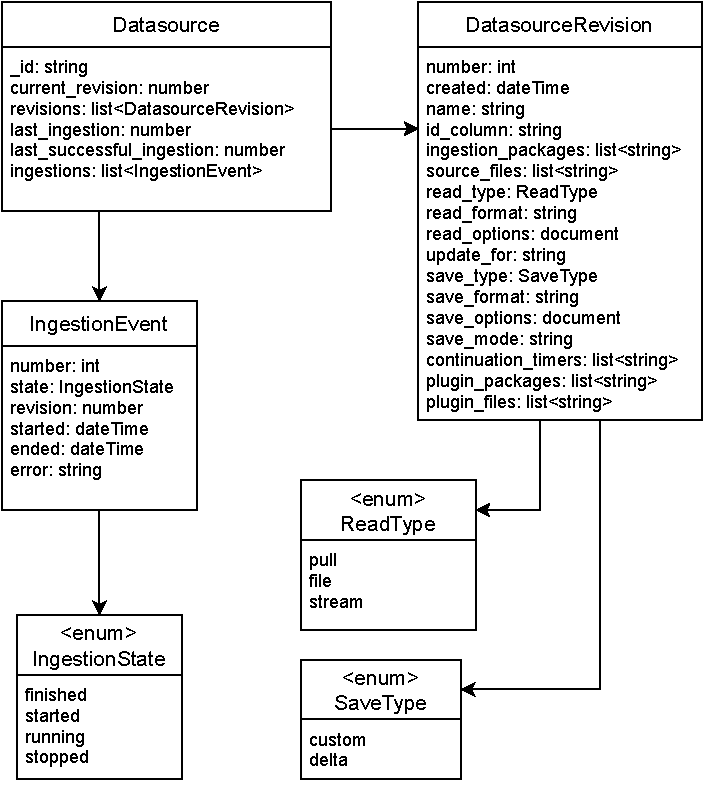
\includegraphics{Grafiken/ingestion-Datamodel.pdf}
    \caption{Datenmodell der Datenquelle}
    \label{fig:datasource_model}
\end{figure}

\subsection{Api-Server}

Da auch das Masterprojekt eine REST-Schnittstelle hat, bietet es sich an, diesen Server so zu erweitern, dass er als Api-Server für das neue System fungiert.
Um die neuen Endpunkte in die aktuelle Lösung zu integrieren, werden die existierenden Pfade, bis auf die zur Authentifizierung, nach "`/api/v1/"' verschoben und die neuen unter "`/api/v2/"' eingefügt.
Auf Grund der Tatsache, dass das neue System mit einem eigenen Datenmodell arbeitet, ist damit die Integration bereits abgehandelt, es muss nur darauf geachtet werden, die Funktionen der beiden Versionen zu trennen.
Die Endpunkte werden mit ihren Funktionen, wie in \fref{sec:arch} beschrieben, implementiert.

Bei der Erstellung und dem Aktualisieren von Datenquellen werden jedes mal eine neue Revision 
Dabei muss besonders darauf geachtet werden, dass bei jeder Änderung einer \verb|Datasource| eine neue \verb|DatasourceRevision| angelegt wird.
Die Quell- oder Plugindateien werden zentral im \textit{HDFS} jeweils einem Unterordner pro Datenquelle abgelegt.
So sind die Dateien von überall aus erreichbar und können auch bei replizierten oder verteilten Microservices verwendet werden.


\subsection{Ingestion-Server}



\subsection{Continuation-Server}

\section{Deltaerkennung}

\section{Datenversionierung}